%Schriftgröße, Dokumentformat, Dokumenttyp
\documentclass[11pt,a4paper]{article}
%Einstellungen der Seitenränder
\usepackage[left=3cm,right=4cm,top=2cm,bottom=2cm,includeheadfoot]{geometry}
%neue Rechtschreibung und Formelsatz
\usepackage[utf8]{inputenc}
\usepackage[english]{babel}
\usepackage[T1]{fontenc}
\usepackage{textcomp}
\usepackage{amsmath,amssymb,amsthm}
%Graphiken
\usepackage{graphicx}
\usepackage{float}
%Zeilenabstand
\usepackage{setspace}\onehalfspacing
%Aufzählungen
\usepackage{paralist}
%Abkürzungen
\usepackage{acronym}
%Tabelle
\usepackage{multirow}
%Kopf- und Fußzeile
\usepackage{fancyhdr}
%Fußnotenkram
\usepackage{footnote}
\usepackage{hyperref}
\usepackage[hang]{footmisc}
\usepackage{graphics}
\usepackage{glossaries}
\setlength{\footnotesep}{0.25 cm}

% HINZUGEFÜGT VON ADRIAN
% MAKE subsubsubsection possible
\usepackage{titlesec}

\usepackage{cleveref}
\usepackage{acronym}

\graphicspath{{./img/}}


% ACRONYMS 
\newacro{GARCH}{General Autoregressive Conditional Heteroskedasticity}
\newacro{ARCH}{Autoregressive Conditional Heteroskedasticity}
\newacro{ARMA}{AutoRegressive Moving Average}
\newacro{SGED}{Skewed Generlized Error Distribution}
\newacro{GED}{Generlized Error Distribution}
\newacro{MSE}{mean-square error}
\newacro{MAE}{mean-absolute error}
\newacro{RMSE}{root-mean-square error}


\setcounter{secnumdepth}{4}

\titleformat{\paragraph}
{\normalfont\normalsize\bfseries}{\theparagraph}{1em}{}
\titlespacing*{\paragraph}
{0pt}{3.25ex plus 1ex minus .2ex}{1.5ex plus .2ex}
%


\begin{document}
% Keine Seitenzahlen im Vorspann
\pagestyle{empty}
	
%%%%%%%%%%%%%%%%%%%%%%% Titelblatt der Arbeit %%%%%%%%%%%%%%%%%%%%%%%
\begin{titlepage}				
	\begin{center}
Professorship for XXX\\
Institute of XXX\\
Faculty of Business, Economics and Social Sciences\\
Kiel University \\
		\vspace{5cm}
		
		\LARGE{ \bf{Density Forecasts of the S\&P using Markov-Switching Models}}
		\vspace{2cm}
		
		\large{\bf{Seminar paper}}\\
		Submission Date: XX.XX.XXXX
		\vspace{1.5cm}

\begin{flushleft}
\vfill
	Author: Adrian Beer
	Subject:\\
	Semester:3
	Module: Seminar in Econometrics
	Stu-Email-Adress:\\
	Matriculation number:\\
	\vspace{1cm}
	First Assessor:\\
	Second Assessor:
\end{flushleft}	
		
				
	\end{center}

\end{titlepage}


%%%%%%%%%%%%%%%%%%%%%%% Inhaltsverzeichnis %%%%%%%%%%%%%%%%%%%%%%%


\newpage
	\tableofcontents
	\newpage


% Kopf- und Fußzeile definieren 
\pagestyle{fancy}					
\fancyhf{}								
%Kopfzeile rechts bzw. außen			
\fancyhead[R]{}							 
%Linie oben								 
\renewcommand{\headrulewidth}{0pt}	 
%Fußzeile mittig					 
\fancyfoot[R]{\thepage}				 
%Linie unten										
\renewcommand{\footrulewidth}{0pt}	 
%Seitenzahlen ab hier						 
\pagenumbering {Roman} 
\setcounter{page}{1}



%%%%%%%%%%%%%%%%%%%%%%%%%%%%% List of Figures %%%%%%%%%%%%%%%%%%%%%%%%%%%%%%%%%
\addcontentsline{toc}{section}{Figure directory}
\listoffigures


\newpage
%%%%%%%%%%%%%%%%%%%%%%%%%%%%% List of Tables %%%%%%%%%%%%%%%%%%%%%%%%%%%%%%%%%
\addcontentsline{toc}{section}{Table directory}
\listoftables
\newpage

%%%%%%%%%%%%%%%%%%%%%%%%%%%%% List of Symbols %%%%%%%%%%%%%%%%%%%%%%%%%%%%%%%
\section*{List of Symbols} 
\addcontentsline{toc}{section}{Symbol directory}
\noindent Include a symbol directory if you use more than three uncommon abbreviations.
	\begin{tabular}{l l}
		\textbf{} & \\
		$\pi$ & rate of inflation\\
		$i$ & nominal interest rate \\
		$r$ & real interest rate \\
		$M$ & money stock \\


	\end{tabular}\\ \vspace{1cm}


\newpage


% Kopf- und Fußzeile definieren %%
\pagestyle{fancy}						
\fancyhf{}								
%Kopfzeile rechts bzw. außen			
\fancyhead[R]{}							 
%Linie oben								 
\renewcommand{\headrulewidth}{0pt}	 
%Fußzeile mittig					 
\fancyfoot[R]{\thepage}				 
%Linie unten										
\renewcommand{\footrulewidth}{0pt}	 
%Seitenzahlen ab hier						 
\pagenumbering {arabic}
\onehalfspacing	
\section{Introduction}
Markov chain processes can be useful for identifying regimes in the past as well as estimating the current regime. %% why is this important
If the Markov model describes the data generating process well, it can also be used to simulate synthetic time series and potential future paths. %% why is this important

\section{Background}

There are two main ways to learn the parameters of a HMM model: Expectation-Maximization Algorithms (EM) such as Baum-Welch. And Markov Chain Monte Carlo methods (MCMC) such as the Metropolis-Hastings or Gibbs Sampling algorithm.

The EM Algorithm makes use of the forward-backward algorithm.

Given a HMM model we can deduce estimates of the hidden state via the Viterbi algorithm.

Our goal is to maximize the incomplete data log-likelihood 
$$\log f(y \mid X ; \theta)=\log \sum_{s_{1}=1}^{2} \sum_{s_{2}=1}^{2} \ldots \sum_{s_{T}=1}^{2} f(y, s \mid X ; \theta)$$ which is not feasible to compute (complexity).


$$ \mathcal{L}\left(\Psi \mid \mathcal{I}_T\right) \equiv \prod_{t=1}^T f\left(y_t \mid \Psi, \mathcal{I}_{t-1}\right) $$ 
\subsection{Markov-Switching Models}

\subsubsection{Exogeneous Variables}
\paragraph{Time-varying transition probabilities}
Most HMMs are trained based on an purely endogeneous variables. One way to introduce exogeneous variables X into the HMM is by using them to estimate time-varying transition probabilities. This concept has been introduced by Diebold et al. \cite{diebold_regime_1993} together with closed form solutions for Gaussian state probability distributions. Since the complexity of calculating the expected likelihood for the EM algorithm in this setting is squared in the number of observations, maximizing it numerically with respect to the parameters is computationally not feasible. Since no closed form solutions to the maximization step for any fat-tailed distributions are available in this setting, this is currently not suited to model financial market data.

\paragraph{State-space model/ DFM-MSs}
Another way to integrate outside information is to use state space models. In this setting the state is represented by one or more so called dynamic factors whose behaviour is specified in the state equation and its relation to the variable of interest in the output equation. The usefulness of this approach depends on two factors: the dynamic factor has to be somewhat predictable and 
needs to explain the output variable reasonably well. The state space model can be learned using the Kalman filters in Gaussian settings or using MCMC methods otherwise.

\subsection{Financial Market Data}

\subsubsection{Stylized Facts about returns and volatility}
Volatility is standard deviation of the log returns.
Fat-tailed. Power-law. Daily vs Monthly frequencies. 

\subsubsection{Heavy-tailed Distributions}
Many different distributions have been suggested for modeling asset returns, among them the log-normal, students-t and the \ac{GED} and stable tempered distributions.
In this paper we will use the \ac{GED}, given the difficulty of implementing algorithms using more advanced distributions such as the stable tempered.
$$f_{\mathrm{GED}}(\eta ; \nu) \equiv \frac{\nu e^{-\frac{1}{2}|\eta / \lambda|^\nu}}{\lambda 2^{(1+1 / \nu)} \Gamma(1 / \nu)}, \quad \lambda \equiv\left(\frac{\Gamma(1 / \nu)}{4^{1 / \nu} \Gamma(3 / \nu)}\right)^{1 / 2}$$

\subsubsection{GARCH}
\label{sss:GARCH}
The \ac{GARCH} model has been popular in order to forecast the volatility of indices. It was introduced  by Bollerslev \cite{bollerslev_generalized_1986} and is an extension of the ARCH model, which was introduced Engle \cite{engle_autoregressive_1982}. It models the error by using a \ac{ARMA} model.
It tries to explain the observation that the volatility of financial assets tends to be heteroskedastic and cluster, i.e. periods with high volatility are followed by periods with high volatility.

The general Markov-switching GARCH specification we use follows \cite{ardia_markov-switching_2019}: 
Denote $y_t$ the log-returns in time period $t$, i.e. $log(p_t-p_{t-1})$ if $p_t$ is the asset price at time t.

$$y_{t} \mid\left(s_{t}=k, \mathcal{I}_{t-1}\right) \sim \mathcal{D}\left(0, h_{k, t}, \xi_{k}\right)$$

$\mathcal{D}$ being some zero-mean distribution, the conditional variance$h_{k,t}$ in state $k$ at time $t$ and shape parameters $\xi$. For short time-periods the zero-mean specification is justified most of the time.  $s_t$ is the state at time t is modeled by a Markov chain.\\

A GARCH(1,1) model has the form $h_{k, t} \equiv \alpha_{0, k}+\alpha_{1, k} y_{t-1}^{2}+\beta_{k} h_{k, t-1}$ models the conditional variance process. $h_{k,t}$ is the conditional variance. Similar to an \ac{ARMA} model which tries specify the conditional mean, the \ac{GARCH} model tries to specify the conditional variance. The lagged squared return term can be interpreted as a proxy for the realized variance in the last observation period. 
In this model long periods of high variance can be modeled by increasing the intercept $\beta$.\\

Many extensions of the GARCH model exist which try to account for the the observation that the variance caused by positive returns don't have the same effect as variance that is caused by negative returns. One example is the GJR model by \cite{glosten_relation_1993}: $$ h_{k, t} \equiv \alpha_{0, k}+\left(\alpha_{1, k}+\alpha_{2, k} \mathbb{I}\left\{y_{t-1}<0\right\}\right) y_{t-1}^2+\beta_k h_{k, t-1}$$

However the GARCH model fails to explain many phenomena which are observed, like the fat-tailedness of drawdown periods and depths (cite Robert Frey).

\section{First chapter of main text}
We try to predict S\&P index using 

\subsection{Experiment description}
We compare the performance of 2 models a stand-alone GARCH model and a MSGARCH model

For the GARCH as well as for the MSGARCH models we will use a \ac{SGED} to describe the distribution of the log-returns.
Also, GJR-GARCH is used for both of the models, see \cref{sss:GARCH}.

\subsubsection{Performance Measures}
When measuring the performance one has to be careful not to compare the square root variance forecasts $\sqrt{h_t}$ with the absolute returns $\sqrt{y_t^2} = | y_t |$ as these would be biased due to Jensen's inequality: Our model tries to achieve $\mathbb{V}(y) =\mathbb{E}(y^2) = h$ and $\mathbb{E}(| y |) \neq \sqrt{h}$. Instead the variance $h_t$ should be compared to the squared returns $y_t^2$.

The actual measures we employ are the following: \ac{MSE}, \ac{MAE}, \ac{RMSE}

\subsection{Data set}
The GARCH model assumes that the datapoints are equidistant in the time dimension, hence we will use the closing prices of the Index and model the close-to-close variance.

We split our dataset s.t. we use the first 80\% observations for training and the last 20\% for testing the models.


\subsection{Results}
\subsubsection{Analysis of Model Parameters}
In \cref{tab:model-params} the model parameters are displayed, which were fitted using a maximum likelihood estimator and the training set.

% latex table generated in R 4.1.2 by xtable 1.8-4 package
% Thu Sep 22 19:29:22 2022
\begin{table}[ht]
\label{tab:model-params}
\centering
\begin{tabular}{rrrr}
  \hline
 & MSSR1 & MSSR2 & GARCH \\ 
  \hline
$\alpha\_1$ & 0.17 & 0.00 & 0.01 \\ 
  alpha1\_1 & 0.02 & 0.02 & 0.03 \\ 
  alpha2\_1 & 0.21 & 0.08 & 0.08 \\ 
  beta\_1 & 0.75 & 0.94 & 0.92 \\ 
  nu\_1 & 1.05 & 1.53 & 6.19 \\ 
  xi\_1 & 0.86 & 0.96 & 0.93 \\ 
   \hline
\end{tabular}
\end{table}




\subsubsection{Evaluation of Point Forecasts}


\begin{table}[ht]
\centering
\begin{tabular}{rrrrr}
  \hline
 & mse & mae & rmse & bias \\ 
  \hline
MSGARCH\_h1 & 24.2096 & 1.5169 & 4.9203 & 0.0195 \\ 
  GARCH\_h1 & 24.9891 & 1.5415 & 4.9989 & 0.0441 \\ 
  MSSR1\_h1 & 25.2808 & 1.5446 & 5.0280 & 0.0380 \\ 
  MSSR\_h1 & 25.2808 & 1.5446 & 5.0280 & 0.0380 \\ 
  Avg & 33.6508 & 1.8815 & 5.8009 & -0.0301 \\ 
   \hline
\end{tabular}
\end{table}

\begin{figure}[h]
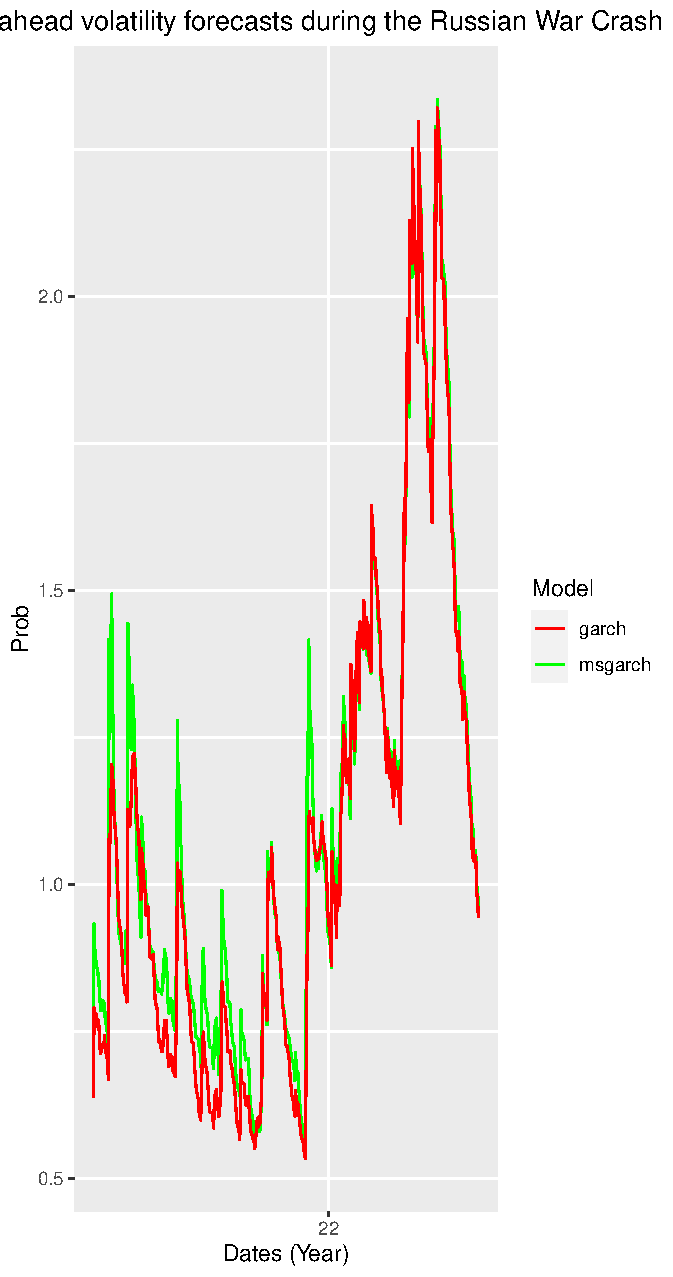
\includegraphics[width=0.8\linewidth]{pforecast-russia-crash.pdf}
\caption{One-day-ahead volatility forecasts during the Corona crash 2020.}
\end{figure}

\begin{figure}[h]
\includegraphics[width=1.2\linewidth]{FiltVola\_InSample\_Eighties.pdf}
\caption{One-day-ahead volatility forecasts during the Corona crash 2020. MSGARCH is model mostly in state 1.}
\end{figure}

\begin{figure}[h]
\includegraphics[width=1.2\linewidth]{CoronaCrash\_MSGARCH\_Decomposition.pdf}
\caption{One-day-ahead volatility forecasts during the Corona crash 2020. MSGARCH is model mostly in state 1.}
\label{img:cor-decomp}
\end{figure}

In \cref{img:cor-decomp} one can see the two states of the MSGARCH (MSSR1 and MSSR2) model produce different forecasts and how they compare to the stand-alone GARCH model. 
It can be observed that MSSR1 is less persistent, which is due to the smaller $\beta_1 = 0.7519$ compared to the larger $\beta_2 = 0.935$ of MSSR2.
Furthermore we see that MSSR1 has a higher base-level volatility and tends to forecast volatility spikes which are larger than those of MSSR2. This once again, is caused by the larger $\alpha$ values which characterise MSSR1.

\section{Conclusion}


\newpage


% Kopf- und Fußzeile definieren 
\pagestyle{fancy}						
\fancyhf{}								
%Kopfzeile rechts bzw. außen			
\fancyhead[R]{}							 
%Linie oben								 
\renewcommand{\headrulewidth}{0pt}	 
%Fußzeile mittig					 
\fancyfoot[R]{\thepage}				 
%Linie unten										
\renewcommand{\footrulewidth}{0pt}	 
%Seitenzahlen ab hier						 
\pagenumbering {Roman} 
\setcounter{page}{5}
\newpage\clearpage

\newpage
\addcontentsline{toc}{section}{Bibliography}
\section*{Bibliography}
In the bibliography, you list all the sources that you use and therefore cite in the text (sources that you have read but not cited should not be listed). Sort the entries in the bibliography, listed according to a consistent style, alphabetically by last name.

\bibliography{References}
\bibliographystyle{Alpha}


\newpage

\begin{flushright}
$\overline{~~~~~~~~~~~~~~~\mbox{(Date, Signature)}~~~~~~~~~~~~~~~}$
\end{flushright}
\end{document}